%!TEX root = ./template-skripsi.tex

\subsection{\textit{Sprint 1}}

	\textit{Sprint-1} dilakukan sepekan pada tanggal 23 Agustus 2022 sampai dengan 30 Agustus 2022. \textit{Story} pertama pada \textit{product backlog} yaitu membuat halamn dashboard dipecah menjadi beberapa \textit{task} sebagai berikut.


 \begin{longtable}[c]{@{} |p{1cm}|p{4cm}|p{5cm}|p{3cm}| @{}}
 \caption{\textit{Sprint 1} \label{sprint1_table}}\\


 \hline
  \multirow{1}{=}{\centering{\textbf{No}}} & \multirow{1}{=}{\centering{\textbf{\textit{Story}}}} & \multirow{1}{=}{\centering{\textbf{\textit{Task}}}} & \multirow{1}{=}{\centering{\textbf{\textit{Status}}}}\\
 \endfirsthead

 \hline
  \multirow{1}{=}{\centering{\textbf{No}}} & \multirow{1}{=}{\centering{\textbf{\textit{Story}}}} & \multirow{1}{=}{\centering{\textbf{\textit{Task}}}} & \multirow{1}{=}{\centering{\textbf{\textit{Status}}}}\\
 \endhead

 \hline
 \endfoot

 \hline
 \endlastfoot

 \hline
 1 & Membuat Halaman Dashboard &  Membuat \textit{Mock-up UI} halaman dashboard  &  selesai \\
 \hline
 2 & & Menerapkan struktur direktori dan membuat class diagram & selesai\\
 \hline
 3 & & Menerapkan \textit{Mock-up UI} halaman dashboard ke Flutter & selesai\\
 \hline
 4 & & Mengintegrasikan halaman home ke \textit{webservice} & selesai\\
 \hline
 \end{longtable}

Pada sprint pertama ini story yang di pilih untuk di uraikan pada sprint kali ini adalah membuat halaman dashboard. Tujuan dari \textit{sprint-1} ini adalah membuat halaman home dan mengintegrasikan halaman tersebut dengan webservice yang sudah dibuat oleh penelitian Andri Rahmanto. Kendala yang dialami penilis pada sprint kali ini adalah diperlukannya waktu traning terhadap bahasa pemrograman dan framework yang digunakan dalam melakukan pengembangan aplikasi,  penulis menggunakan \textit{GitHub Projects} seperti pada gambar \ref{gambar:sprint1_projects}.
	
\begin{figure}[H]
	\centering
	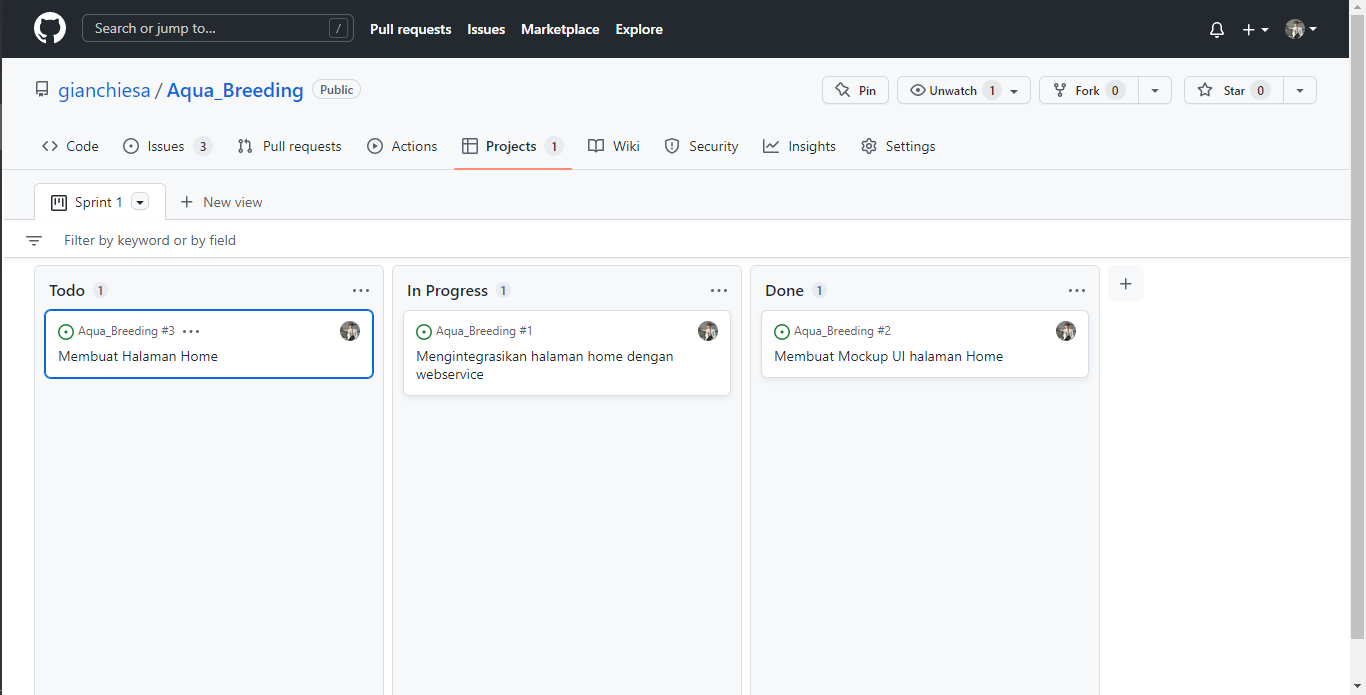
\includegraphics[keepaspectratio, width=14cm]{gambar/githubprojectgian}
	\caption{\textit{Github Projects Sprint-1}}
	\label{gambar:sprint1_projects}
\end{figure}
	
Terdapat 3 kolom pada \textit{project} yang dibuat, yaitu \textit{to do}, \textit{in progress}, dan \textit{completed}. Setiap \textit{task} yang perlu dikerjakan akan ditulis dan dimasukkan ke dalam kolom \textit{to do}, selanjutnya \textit{task} yang sedang dikerjakan akan dipindahkan ke kolom \textit{in progress}, dan jika task sudah selesai akan dipindahkan ke kolom \textit{completed}. Berikut merupakan hasil dari pengerjaan yang dilakukan selama \textit{sprint 1}.

\begin{enumerate}[listparindent=2em]
	
	\item{\textit{Membuat Mock-up UI Halaman Dashboard}}
	
	Pembuatan konten dan fitur yang terdapat pada \textit{mock-up UI} halaman home dilakukan berdasarkan persetujuan product owner dan scrum master pada meeting sebelumnya. Mock-up UI dibuat menggunakan platform figma.
	
	\begin{figure}[H]
	\centering
	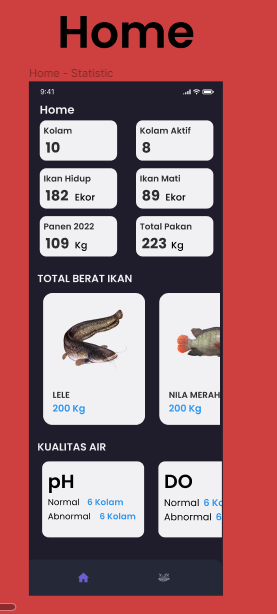
\includegraphics[keepaspectratio, width=4cm]{gambar/mockuphome}
	\caption{\textit{Mock-up UI Halaman Dashboard}}
	\label{gambar:mockuphome}
	\end{figure}

	Lalu selanjutnya dibuat prototype agar product owner dan scrum master dapat lebih mengerti bagaimana konten dan fitur tersebut berjalan saat akan dikembangkan seperti pada gambar \ref{gambar:protohome}.

	\begin{figure}[H]
	\centering
	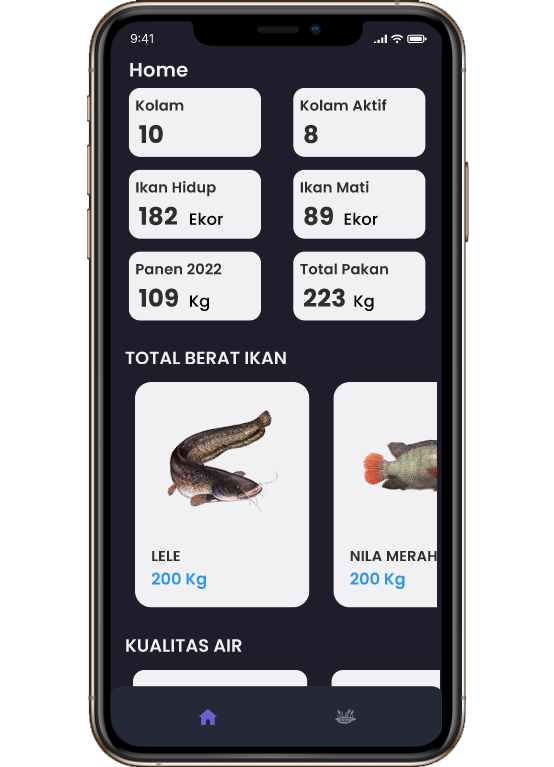
\includegraphics[keepaspectratio, width=5cm]{gambar/protohome}
	\caption{\textit{Prototype Halaman Dashboard}}
	\label{gambar:protohome}
	\end{figure}
	
	\item{\textit{Menetapkan Struktor Direktori}}

	Sebelum menerapkan Mockup-UI kedalam code, penulis membuat atau menetapkan struktur direktori file agar memudahkan penulis untuk melakukan proses pengembangan untuk kedepannya. Terdapat 4 direktori yang penulis buat pada penelitian kal ini, yaitu models, controllers, pages, dan services. Direktori models akan memuat file yang berfungsi sebagai model class, lalu pada direktori contoller berisi file controller-controller yang akan digunakan pada suatu halaman/fitur untuk memanipulasi/mengolah data yang didapat dari services. Direktori services berisi file yang digunakan untuk berinteraksi dengan dunia luar seperti pemanggilan API dan membuat network request, untuk direktori pages memuat file UI halaman.

	\begin{figure}[H]
	\centering
	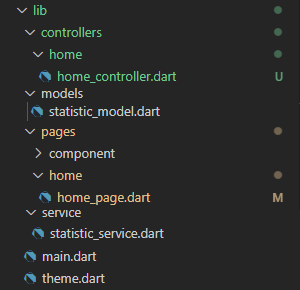
\includegraphics[keepaspectratio, width=7cm]{gambar/homedirektori}
	\caption{\textit{Struktur Direktori}}
	\label{gambar:homedirektori}
	\end{figure}

	\item{\textit{Class Diagram}}
	
	Class Diagram menggambarkan kelas-kelas yang akan dipakai oleh sistem. Umumnya terdapat 3 kelas pada setiap module yaitu class model, controller, dan view. Pada sprint-1 penelitian kali ini penulis membuat 4 class yaitu model, view , controller, dan service.
	 
	\begin{figure}[H]
	\centering
	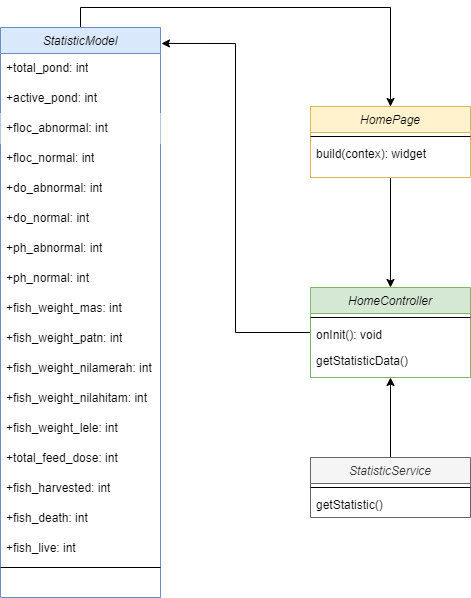
\includegraphics[keepaspectratio, width=6cm]{gambar/CDfishnew}
	\caption{\textit{Class Diagram Sprint-1}}
	\label{gambar:classdiagram}
	\end{figure}

	Pada gambar \ref{gambar:classdiagram} class HomePage sebagai view menginisiasi controller dari interaksi dengan user, lalu controller akan memanggil mengfetch data dari service class dan memasukan data tersebut ke model class, setelah itu model class akan memberi tahu sistem jika data sudah terupdate dan akan mengirimkan data tersebut kembali ke view.

	\item{\textit{Menerapkan Mockup-UI Halaman Dashboard kedalam code flutter}}
	
	Setelah \textit{mock-up UI Halaman Dashboard} hingga prototype dibuat, akan dilakukan pengimplementasian \textit{mock- up UI} ke dalam aplikasi menggukan flutter. Pada lampiran 2 terdapat source code dari implementasi halaman home yang dikelompokan berdasarkan section.

	\item{\textit{Mengitegrasikan Halaman Dashboard dengan webservice}}
	
	Sebelumnya, setiap data pada halaman home masih berupa data dummy sehingga perlu diintegrasikan dengan webservice agar aplikasi dapat berjalan dengan data yang asli. pada lampiran 6 terdapat langkah-langkah untuk mengintegrasikan halaman dashboard dengan webservice.
	

\item{Sprint 1 Review dan Sprint 2 Planning}

Sprint 1 diakhiri dengan melakukan weekly meeting pada hari selasa dengan agenda melakukan review dan testing terkait hasil sprint 1 dan melakukan planning untuk sprint 2 dengan rincian:
\begin{enumerate}
	\item{\textit{Review dan Testing hasil dari sprint 1}}

	Telah dilakukan review dan testing oleh penulis selaku developer dengan Scrum Master. Setelah dilakukan testing, Scrum Master menyimpulkan bahwa fitur pada halaman dashboard telah berjalan dengan baik.

	\begin{longtable}{| p{8cm} | c | c | l |}
		\caption{Unit testing Halaman Dashboard.\label{table:unit_testing_fitur_dashboard}}\\
		\hline
		\multirow{2}{*}{Skenario Pengujian} & \multicolumn{2}{l|}{Kesesuaian} & \multirow{2}{*}{Kesimpulan} \\ 
		\cline{2-3}
		  & \multicolumn{1}{l|}{sesuai} & tidak sesuai & \\ 
		\hline
		\hline
		\endfirsthead
		\hline
		\multirow{2}{*}{Skenario Pengujian} & \multicolumn{2}{l|}{Kesesuaian} & \multirow{2}{*}{Kesimpulan} \\ 
		\cline{2-3}
		  & \multicolumn{1}{l|}{sesuai} & tidak sesuai &  \\ 
		\hline
		\hline
		\endhead
		\hline
		\endfoot
		
		
		\hline\hline
		\endlastfoot
		 Ketika mengisi form login dengan data yang sesuai kemudian menekan submit, maka akan masuk ke halaman dashboard & \Checkmark &  & Diterima \\ 
		\hline
		 Saat tombol kolam ditekan maka akan muncul halaman yang menampilkan list kolam & \Checkmark & & Diterima \\ 
		\hline
		\end{longtable}

	\begin{figure}[H]
	\centering
	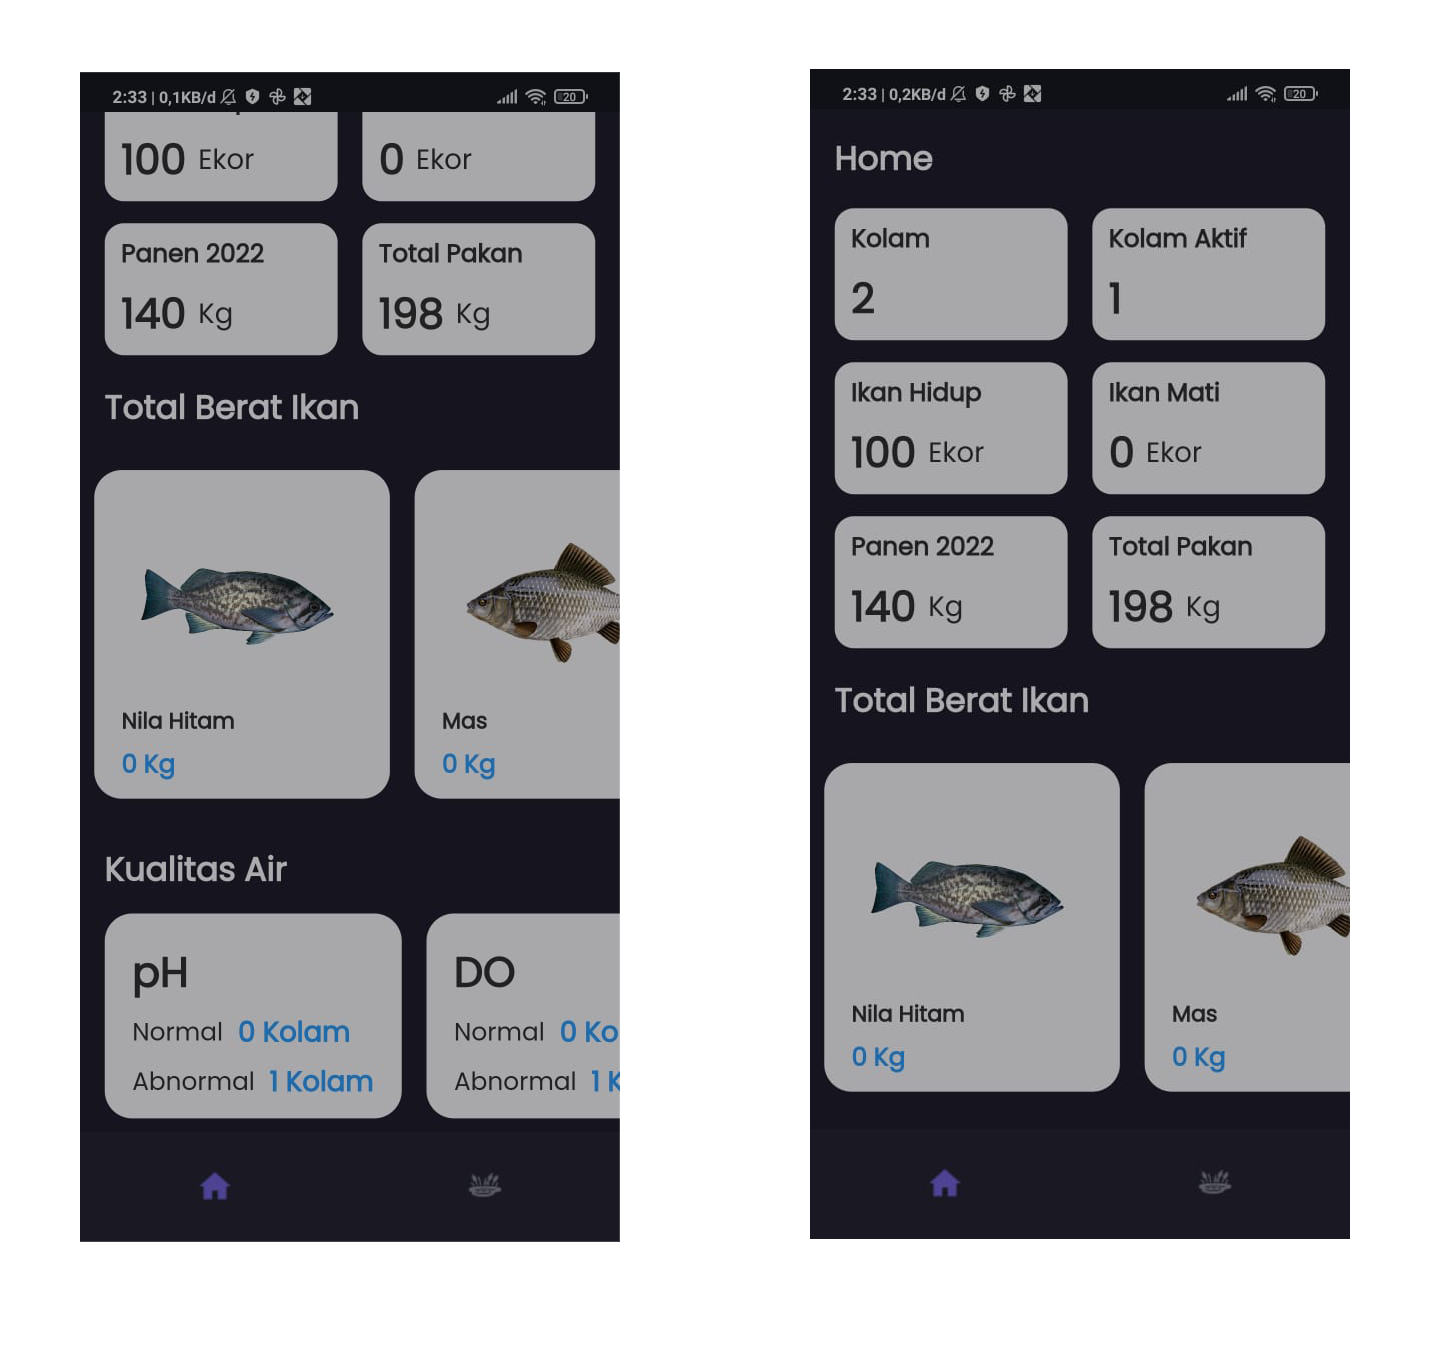
\includegraphics[keepaspectratio, width=7cm]{gambar/ssaqua}
	\caption{\textit{Screenshot dari Halaman Home yang telah selesai}}
	\label{gambar:mockuphome}
	\end{figure}

	\item{\textit{Sprint Planning untuk Sprint 2}}
	
	Planning untuk sprint 2 yakni membuat fitur registrasi kolam dan aktifasi musim budidaya pada aplikasi \textit{Assistive Aquaculture Breeding Management}.
\end{enumerate}
\end{enumerate}
`	